%%%%%%%%%%%%%%%%%%%%%%% file template.tex %%%%%%%%%%%%%%%%%%%%%%%%%
%
% This is a general template file for the LaTeX package SVJour3
% for Springer journals.          Springer Heidelberg 2010/09/16
%
% Copy it to a new file with a new name and use it as the basis
% for your article. Delete % signs as needed.
%
% This template includes a few options for different layouts and
% content for various journals. Please consult a previous issue of
% your journal as needed.
%
%%%%%%%%%%%%%%%%%%%%%%%%%%%%%%%%%%%%%%%%%%%%%%%%%%%%%%%%%%%%%%%%%%%
%
% First comes an example EPS file -- just ignore it and
% proceed on the \documentclass line
% your LaTeX will extract the file if required
%\begin{filecontents*}{example.eps}
%!PS-Adobe-3.0 EPSF-3.0
%%BoundingBox: 19 19 221 221
%%CreationDate: Mon Sep 29 1997
%%Creator: programmed by hand (JK)
%%EndComments
%gsave
% newpath
%   20 20 moveto
%   20 220 lineto
%   220 220 lineto
%   220 20 lineto
% closepath
% 2 setlinewidth
% gsave
%   .4 setgray fill
% grestore
% stroke
% grestore
% \end{filecontents*}
% %
% \RequirePackage{fix-cm}
%
%\documentclass{svjour3}                     % onecolumn (standard format)
%\documentclass[smallcondensed]{svjour3}     % onecolumn (ditto)
\documentclass[smallextended,natbib]{svjour3}       % onecolumn (second format)
%\documentclass[twocolumn]{svjour3}          % twocolumn
%
\smartqed  % flush right qed marks, e.g. at end of proof
%
\usepackage{amsmath}
\usepackage{booktabs}
\usepackage[T1]{fontenc}
\usepackage[utf8]{inputenc}
\usepackage{float}
\usepackage{graphicx}
\usepackage{booktabs}
\usepackage{enumitem}
\usepackage[hyphens]{url}
%\usepackage{cite}
%
% \usepackage{mathptmx}      % use Times fonts if available on your TeX system
%
% insert here the call for the packages your document requires
%\usepackage{latexsym}
% etc.
%
% please place your own definitions here and don't use \def but
% \newcommand{}{}
%
% Insert the name of "your journal" with
% \journalname{myjournal}
%
\begin{document}

\title{Evaluation of LoRaWAN Transmission Range for Wireless Sensor Networks in Riparian Forests%\thanks{Grants or other notes
%about the article that should go on the front page should be
%placed here. General acknowledgments should be placed at the end of the article.}
}
%\subtitle{Do you have a subtitle?\\ If so, write it here}

%\titlerunning{Short form of title}        % if too long for running head

\author{Pablo Avila-Campos \and \\Fabian Astudillo-Salinas \and \\Andres Vazquez-Rodas \and \\Alcides Araujo}

%\authorrunning{Short form of author list} % if too long for running head

\institute{Universidad de Cuenca / Department of Electric, Electronics and Telecommunications \at
              12 de Abril S/N, Cuenca-Ecuador \\
              Tel.: +593-7-4051000\\
              \email{\{pablo.avila, fabian.astudillos, andres.vazquezr, alcides.araujo\}@ucuenca.edu.ec}           %  \\
%             \emph{Present address:} of F. Author  %  if needed
}

\date{Received: date / Accepted: date}
% The correct dates will be entered by the editor


\maketitle

\begin{abstract}
Low power wide area networks (LPWAN) such as long range wide area networks (LoRaWAN), provide several advantages to develop monitoring systems in forested environments due to its simple set-up, low cost, low power consumption, and wide coverage. Regarding the coverage area, the transmission in forested environments can be highly attenuated by foliage and must be defined to optimize the number of nodes. This paper discusses an empirical study of LoRa with LoRaWAN transmission range in riparian forests, based on path-loss modeling, using both received signal strength indicator (RSSI) and signal-to-noise-ratio (SNR). The measurements have been conducted in the riparian forest of three local rivers located at urban, semi-urban and rural environments in the city of Cuenca, Ecuador. The measurement results found that there is a significant distribution difference among measurement places, a high correlation between two banks of a same river, a higher standard deviation in urban measurements and a larger coverage in rural areas.

\keywords{LoRa; LoRaWAN, IoT, RSSI, SNR, path loss, forested, riverside, propagation, model, riparian}
% \PACS{PACS code1 \and PACS code2 \and more}
% \subclass{MSC code1 \and MSC code2 \and more}
\end{abstract}

\section{Introduction}
\label{intro}

Program for water and soil management (PROMAS for its acronym in Spanish) monitors a wealth of environmental information regarding wind, rain, temperature, humidity, barometric pressure and water level of rivers. For this, around $130$ remote weather stations have been deployed in a large area of Azuay, Cañar and Chimborazo. PROMAS has two projects related to limnigraphic sensors. The first one is the early flood warning and the other is the flow prediction using neural networks \cite{felipeartificial}. The idea for the last one is to improve the model adding real time information. Currently, the researchers download the data directly at every sensor location.

Our research team is working on the design and implementation of a wireless network to gather the sensors information and transmit it to the PROMAS data center. The goal is to take advantage of wireless technologies to reduce the displacement of people in charge of downloading the data. This, consequently, will maximize the availability of limnigraphic information in an hour-based transmissions, reduce the risk of losing information, and diminish mobilization expenses that can be used for maintenance purposes.

LPWANs represent a new trend in the evolution of wireless telecommunications technologies. This communication technology is able to connect and monitor high number of sensors, covering wide areas at low energy cost \cite{Augustin2016}. One of the newest approaches to this technology is long range (LoRa) \cite{Semtech2015}. LoRa gives all these LPWAN advantages, adding low device cost and easy deployment. These LoRa-based wireless sensor networks (WSNs), are able to collect real time information such as temperature, rain, humidity, flow, and other weather factors. A clear aplication scenario for LoRa is forest environments. About $30\%$ of the world's land surface is covered by forest, and more than $300$ million people live in forest \cite{wwf2016}.

%Projects such as the prediction of water flows in the basin of Tomebamba river made by the \textit{Program for Water and Soil Management} (PROMAS) of the University of Cuenca, is a clear beneficiary of this technology \cite{FabianAstudillo2016}. LoRa can cover the extensive geographic areas needed and transmit the information in real time, thereby reducing the prediction error regard to a latency improvement.

LoRaWAN, created by the LoRa Alliance, is a Medium Access Control layer that uses the advantages of LoRa modulation to create Networks and it is focused on the internet of things (IoT) paradigm \cite{Wixted2017}. LoRaWAN uses a star topology where the nodes, collect the sensor information and send it to the gateways (GW). The GWs convert the data to the internet protocol (IP) and forward it to a remote application server via Internet. This architecture is shown in Fig. \ref{fig:lorawanarchitecture}.

\begin{figure}[h!]
  \centering
  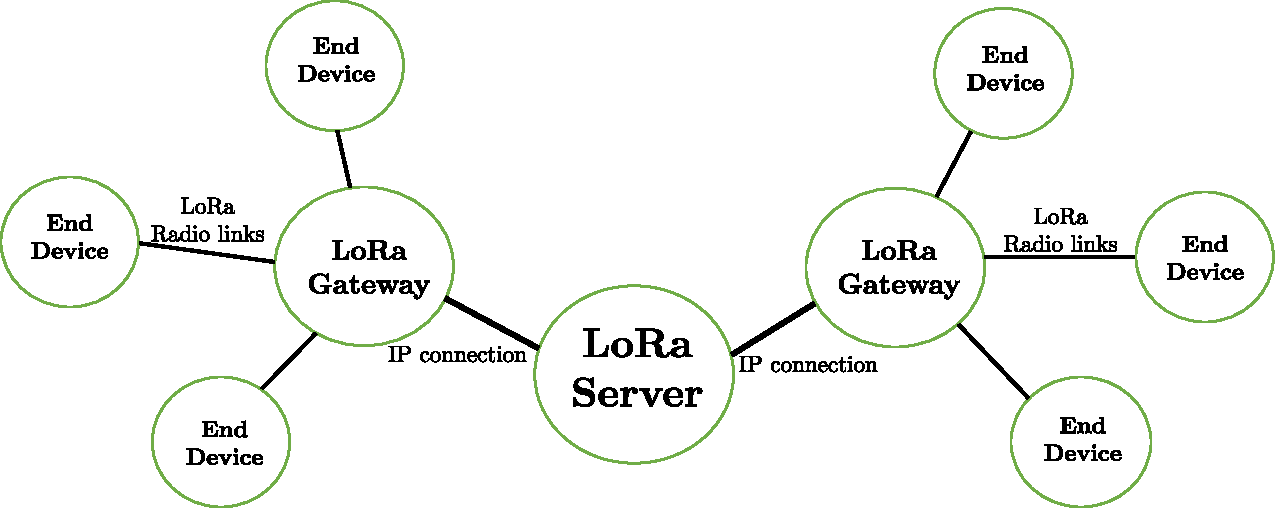
\includegraphics[width=0.9\textwidth]{./figures/Figure1/Figure1.pdf}
  \caption{LoRaWAN Architecture \cite{Vangelista2015}}
  \label{fig:lorawanarchitecture}
\end{figure}


When designing any wireless network, the main question that must be answered is the maximum distance between two nodes that still ensures a reliable wireless connection. Environmental vegetation plays a significant role in the fading phenomena in wireless communications \cite{Meng2008}. The answer also depends on different technical parameters such as the transmitter power, receiver sensitivity, signal propagation and signal frequency \cite{Harvanova2011}. Until now, there are studies reported in the literature about performance, scalability, indoor propagation, and range evaluation, but given that LoRa is a rather new technology, there are no reported measurements of propagation in riparian forest.

%TODO (poner en algún lado): Para realizar el diseño de red, se requiere hacer una primera aproximación, para lo cual se requieren hacer simulaciones. El módelo de propagación usado por LoRaSim es únicamente el path loss y no toma en cuenta los escenarios presentes en el proyecto (básicamente sensores a lado de los rios). Por lo que la primera aproximación es aproximar de la mejor manera modelos de propagación a estos escenarios. Una vez que tengamos los modelos se diseñará la red tomando en consideración los resultados de la simulación.

The contribution of this paper is to present the results of a $915\;$MHz ISM band, LoRa modulation riparian forest propagation measurement campaign. This kind of scenario is present when the limnigraphic stations are used. The main task is to capture channel statistics through received signal strength indicator (RSSI), signal-to-noise ratio (SNR), and packet error rate (PER) under different LoRaWAN available data rates (DR) at a height of under $2\;$m \cite{N.SorninSemtechM.LuisSemtechT.EirichIBMT.KrampIBM2015}.  

To the best of our knowledge, this is the first low antenna height LoRa measurement campaign conducted in a riparian forest. This collected data will be used to adjust a path loss model ($P_L$) to the specific measurement locations \cite{Mikhaylov2016}. This study will help to a faster design and deployment of LoRa sensor networks, making it easier to calculate the useful coverage area of a LoRaWAN system.


\section{Related Work}

In this section, we discuss briefly some of the most important works related to propagation and coverage measurements, made with LoRa.

In \cite{Mikhaylov2016}, the authors present a study of performance and coverage that uses LoRa transceivers and RSSI as the main measurement variable to develop a path loss model. This work differs from our research mainly in two relevant aspects. First, this study is conducted in water and a coast environment. Second, they use European $868\;$MHz ISM band while we use American $915\;$MHz ISM band. This is because our study is conducted in Latin America allowing us to use different channels, and transmission power. 

Another outdoor measurement based study is presented in \cite{Aref2014}, where the authors use PER and RSSI to estimate the performance of the system under two different tests. Authors evaluate the system under different payload length, bandwidth (BW), spreading factor (SF), and modulation schemes. The principal differences with our study are that they use of different payload length, transmission with the FSK modulation scheme, and the Fresnel zone is taken into account.

Another work, \cite{Wixted2017}, presents a general evaluation of LoRa using multiple gateways; RSSI and ACKs to estimate the connection rate. A main aspect of the study is the reliability that was measured using long transmission periods. The study detected mobile network interference during certain hours that in not considered in the current work.

On the other hand, indoor measurements have been conducted in \cite{Gregora2016} and \cite{Petajajarvi2016}. In \cite{Gregora2016}, DR, SF, bandwidth and bit rate are fixed and RSSI is used to measure performance. In \cite{Petajajarvi2016}, the study is more specific, the authors evaluated the performance of LoRa in health and wellbeing applications. The main difference is that we take into account an outside riparian environment of three rivers for measurements.

%==========================================================================================================
%%%%%%%%%%%%%%%%%%%%%%%%%%%%%%%%%%%%%%
\section{Theoretical Background - RSSI and SNR based Path Loss Model}
\label{sec:theory}
In this section, we give a brief review of RSSI and SNR-based propagation models used in this study. Path Loss models are usually expressed in a logarithmic form as shown in Eq. \eqref{eq:1} \cite{Iswandi2017}.

\begin{equation} 
\label{eq:1}
P_L(dB) = P_0(dBm) + 20\;\log\left(\frac{d}{d_0}\right)+X_\theta
\end{equation}  

where $d$ and $d_0$ are the transmission distance and reference distance respectively. $P_0$ is the power strength at $d_0$. $X_\theta$ is a random variable normally distributed with standard deviation $\theta$.

Another widely used model is the exponential decay model, shown in Eq. \eqref{eq:2} \cite{RamaRao2012}. This equation shows that path loss is an exponential function with frequency $f$ and distance $d$. This equation was proposed for cases were the antennas are located near to trees and thus the signal propagates through the trees. Weissberger and COST-$235$ models are modifications of this model to different forested environments.

\begin{equation}
\label{eq:2}
L(dB) = A\; f^{B}d^{C}
\end{equation} 

These models can be simplified into Eq. \eqref{eq:3}, as is proposed in \cite{Iswandi2017}.

\begin{equation}
\label{eq:3}
P_L(dB) = a + b\;\log(d)+X_\theta
\end{equation}

In this case, all the characteristics of Eq. \eqref{eq:2} are expressed in Eq. \eqref{eq:3}. The exponential factor of distance is $b$, and the other are expressed by $a$. As in Eq. \eqref{eq:1}, the randomness of the received signal is expressed in $X_\theta$. It is assumed that the error of fitting in \eqref{eq:3} follows a normal distribution with zero mean and standard deviation ($\theta$). In this work, the standard deviation is calculated between the fitted curve and the mean values of every measurement point as shown in Eq. \eqref{eq:4}.

\begin{equation} \label{eq:4}
\theta = \text{std}(P_L-\text{FittedCurve})
\end{equation}

To calculate the $P_L$ values from RSSI and SNR, Equation \eqref{eq:5} is used according to \cite{Mikhaylov2016}.

\begin{equation} \label{eq:5}
P_L=|\text{RSSI}|+\text{SNR}+P_{\text{tx}}+G_{\text{rx}}
\end{equation}

%%%%%%%%%%%%%%%%%%%%%%%%%%%%%%%%%%%%%%%%%%
\section{Materials and Methods}

This section presents a detailed description about the device parameters, environmental conditions and statistical tests used in the current work.

\subsection{Equipment and Configuration}
Propagation measurements are made at $915\;$MHz utilizing Microchip's Evaluation kit - $900$. The Evaluation kit consist of a gateway working with the LoRa Semtech chip SX$1301$, two nodes that include light and temperature sensors with the RN$2903$. Transmission power, spreading factor, code rate and bandwidth are controlled by the LoRaWAN MAC protocol included \cite{N.SorninSemtechM.LuisSemtechT.EirichIBMT.KrampIBM2015}. The operation Data Rates (DR) can vary from $0$ to $3$ and the maximum power index of $5$ gives a transmission power of $18.5\;$dBm. Technical modulation parameters are shown in Tab. \ref{tab:EquipmentandParameters}. LoRaWAN DRs parameters are shown in Table \ref{tab:datarates}. 

For this experiment we used one node transmitting $10$ numerated messages transmitted with DR$0$, and $10$ messages with DR$3$. The gateway is connected to a virtual server in a laptop to register the RSSI, SNR and the number of received messages at every transmission. Transmitter and receiver were located two meters above ground level. Physical configuration scheme is presented in Fig. \ref{fig:physicalconfig}. The implementation is available in \cite{Avila2017}.

\begin{figure}[h!]
  \centering
  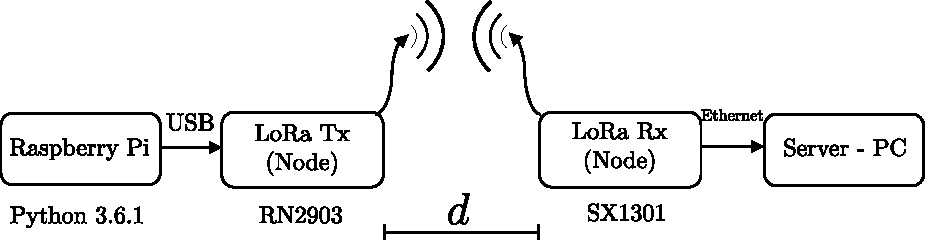
\includegraphics[width=0.9\textwidth]{./figures/Figure2/Figure2.pdf}
  \caption{Equipment Physical Configuration}
  \label{fig:physicalconfig}
\end{figure}


\begin{table}[h!]
  \centering
  \caption{Equipment and Parameters of Transmission \cite{Microchip2016a}}
  \label{tab:EquipmentandParameters}
  \resizebox{8cm}{!} {
    \begin{tabular}{lr}
      \toprule
      \textbf{Parameters/Equipment} & \textbf{Values/Description} \\ 
      \midrule
      Transmitter & RN$2903$\\ 
      Receiver & SX$1301$\\ 
      Antenna Gains & $1.3\;$dBi\\ 
      Modulation & LoRa\\ 
      Spreading Factor & $7-10$\\
      Bandwidth & $125\;$kHz\\ 
      Code Rate & $4/5$\\ 
      Power Level & $18.5\;$dBm\\ 
      \bottomrule
    \end{tabular}
  }
\end{table}


\begin{table}[h!]
  \centering
  \caption{Equipment Data Rates \cite{N.SorninSemtechM.LuisSemtechT.EirichIBMT.KrampIBM2015}}
  \label{tab:datarates}
  \resizebox{9cm}{!} {
    \begin{tabular}{clr}
      \toprule
      \multicolumn{1}{l}{\textbf{Data Rate}} & \textbf{Configuration {[}SF/BW{]}} & \multicolumn{1}{l}{\textbf{Bit Rate {[}bit/sec{]}}} \\
      \midrule
      $0$                             & SF$10 / 125\;$kHz            & $980$                                        \\
      $1$                             & SF$9 / 125\;$kHz             & $1760$                                       \\
      $2$                             & SF$8 / 125\;$kHz             & $3125$                                       \\
      $3$                             & SF$7 / 125\;$kHz             & $5470$                                     \\
      \bottomrule
    \end{tabular}
  }
\end{table}

\subsection{Environment and Measurement Procedure}

In this work, we carried out four measurements in three different locations at the city of Cuenca, Ecuador. The first two measurements were made at the two riversides of Tomebamba river in an urban environment. This zone is characterized by different tree species of heights between $2$ and $6$ meters with irregular separations ranging from $4$ to $6$ meters. The ground in covered with short grass. 
The third measurement were done in one riverside of the Machángara river in a semi-urban zone of the same city. This place have mainly tree species of more than $5$ meters in height, separations from $3$ to $6$ meters. The ground is covered by grass and rocks. The last measurement were done at a rural zone in the riverside of the Yanuncay river. In this zone there are different trees species of heights between $1$ to $6$ meters with irregular separations from $1$ to $4$ meters. All rivers have a width of approximately $10$ meters.

 At each location, measurements were collected using a process called local average power, explained in \cite{Lee1985}. According to this measurement procedure, one has to move a distance $d$ of $20\lambda$ to $40\lambda$ in every measurement. Ten meters was selected in this study with the transmitter moving and the receiver (GW) fixed. As said before, at each point 20 packets were sent and registered by the receiver. Figure \ref{fig:locationmap} shows the sampling points represented by circles and the receiver location represented by the star at the upper left of the map.

\begin{figure}[h!]
  \centering
  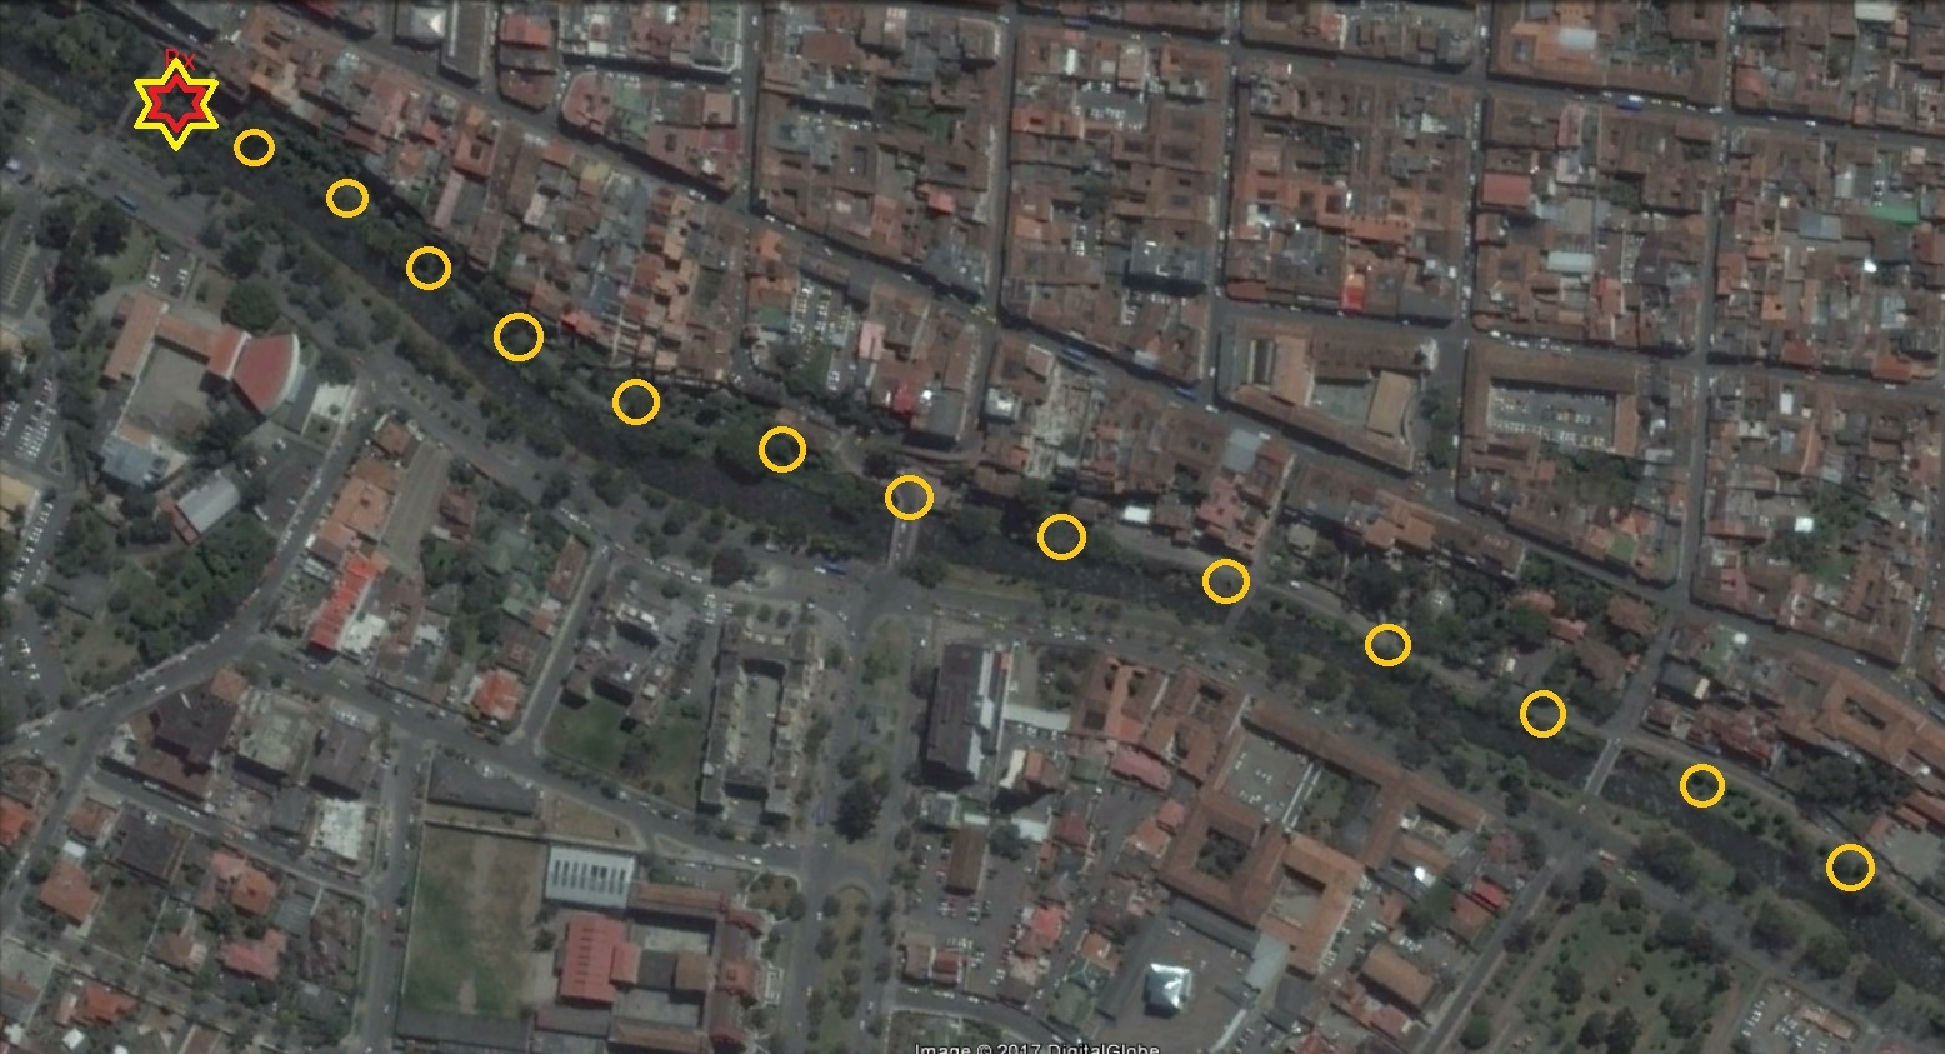
\includegraphics[width=1\linewidth]{map.jpg}
  \caption{Sampling location map - Measurement $1$}
  \label{fig:locationmap}
\end{figure}

\subsection{Statistical Analysis and Fitting}
\label{sub:statistical}
In first place, a correlation analysis was done using the Measurements $1$ and $2$ to prove the relationship between the RSSI values of a same river.
An statistical analysis is done to prove the hypothesis that the urban, semi-urban and rural RSSI measurements follow different distributions. Kruskal-Wallis and Dunn tests are used to prove the hypothesis \cite{Mendenhall2010}. DR$0$ and DR$3$ RSSI means measurements follow a similar distribution as shown in Fig. \ref{fig:rssimeasurement}, for this reason, the tests were performed only with DR$0$.

\begin{figure}[h!]
  \centering
  % \includegraphics[width=1\linewidth]{RSSI.png}
  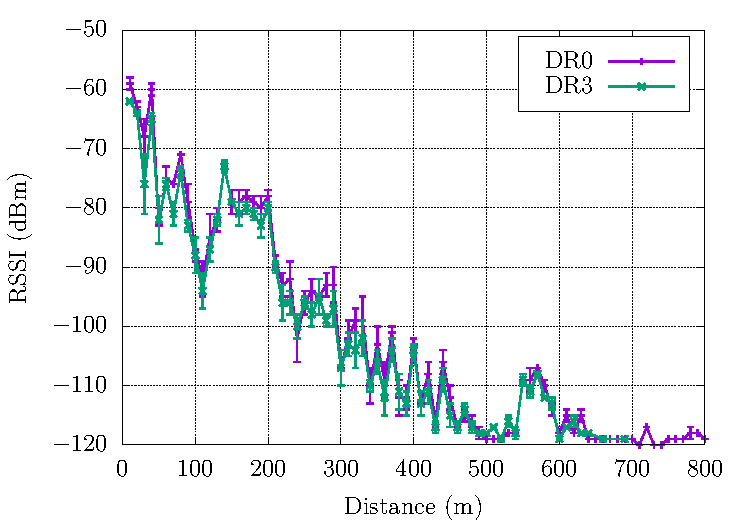
\includegraphics[width=0.9\textwidth]{./figures/Figure4/Figure4.pdf}
  \caption{RSSI measurement 1 with DR$0$ and DR$3$}
  \label{fig:rssimeasurement}
\end{figure}

This study focuses on generating a path loss model based on RSSI and SNR values. Figure \ref{fig:plfittiing} shows the fitting result of the urban environment with the minimum data rate. The empirical model generated is useful to determine the number of required nodes in a riparian forested environment, that uses LoRaWAN and similar technologies.

\begin{figure}[h!]
  \centering
  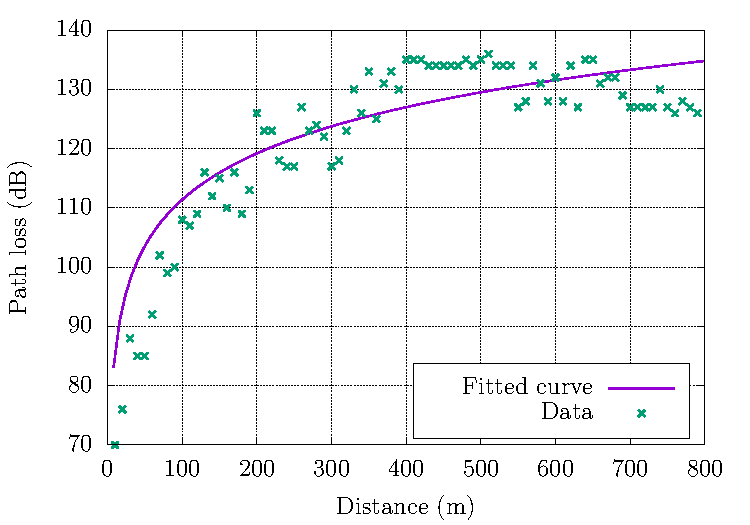
\includegraphics[width=0.9\textwidth]{./figures/Figure5/Figure5.pdf}
%  \includegraphics[width=1.1\linewidth]{3.png}
  \caption{$P_L$ fitting in urban environment with minimum data rate}
  \label{fig:plfittiing}
\end{figure}

%=============================================================================================================
\section{Results and Discussion}

This section discusses and shows the results of measurements of LoRa transmission on different riparian forested environments. In first place, we show the correlation found between the riversides in the urban environment. Then the Kruskal-Wallis, Dunn tests and Path loss fitting results of DR$0$ and DR$3$ are presented. Finally, the variables of maximum coverage and standard deviation are compared between the different measurements.  

\subsection{Previous Measurements}

To find the best number of messages to send at every sampling point, we did previous measurements of RSSI and SNR. Table \ref{tab:stdmessages} shows the standard deviations of RSSI for different number of packets. Standard deviations show an expected tendency to decrease with the increase of sent messages. However, $10$ packets were selected to send at every transmission point due to a low standard deviation variation of about $1\;$dBm. 

\begin{table}[h!]
\centering
\caption{Standard deviation of RSSI with different number of packets}
\label{tab:stdmessages}
\begin{tabular}{@{}ccc@{}}
\toprule
\textbf{Test} & \textbf{Packets} & \textbf{RSSI Standard Deviation (dBm)} \\ \midrule
$1$                    & $10$                     & $1.94$                                \\
$2$                    & $20$                     & $1.16$                                \\
$3$                    & $30$                     & $1.76$                                \\
$4$                    & $40$                     & $1.63$                                \\
$5$                    & $50$                     & $2.06$                                \\
$6$                    & $60$                     & $1.57$                                \\
$7$                    & $70$                     & $1.18$                                \\
$8$                    & $80$                     & $1.10$                                \\
$9$                    & $90$                     & $1.25$                                \\
$10$                   & $100$                    & $1.05$                                \\ \bottomrule
\end{tabular}
\end{table}

\subsection{Statistical Analysis}
In this section, we show the RSSI correlation analysis and Kruskal-Wallis and Dunn analysis results as described in Section \ref{sub:statistical}.

\begin{itemize}
%[leftmargin=!,labelindent=5pt,itemindent=-15pt]

\item \textbf{Correlation Analysis:} It was carried out to know how correlated the RSSI measurements are between the two banks of the same river.
In the case of measurements with the minimum data rate, a correlation value of $0.923$ was obtained. Therefore, it is concluded that the correlation is high. This relationship is shown in Fig. \ref{fig:comparisonrssidr0}.

% \begin{figure}[h!]
%   \centering
%   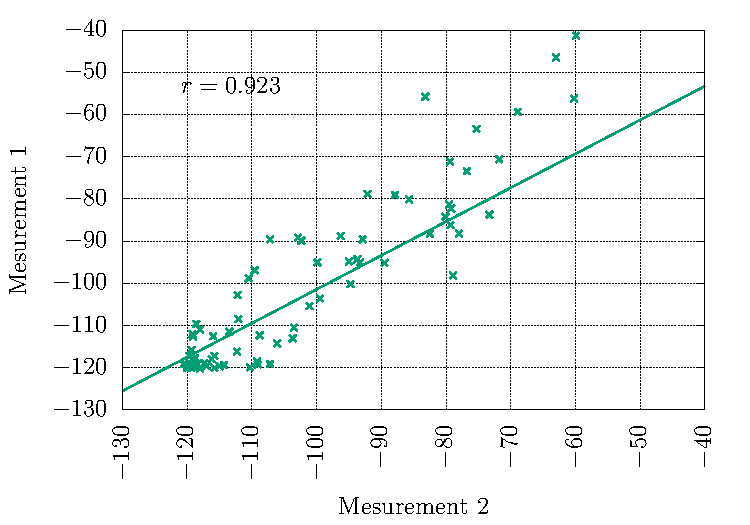
\includegraphics[width=0.8\textwidth]{./figures/Figure6/Figure6.pdf}
% %	\includegraphics[width=0.8\linewidth]{correlation.png}
%   \caption{Comparison of RSSI values at Tomebamba river with DR$0$}
%   \label{fig:comparisonrssidr0}
% \end{figure}

In the same way, in the case of RSSI measurements with the maximum data rate, a correlation coefficient of $0.922$ was obtained, so it is concluded that there is a strong relationship between measurement $1$ and measurement $2$. This is shown in Fig. \ref{fig:comparisonrssidr3}.

% \begin{figure}[h!]
%   \centering
%   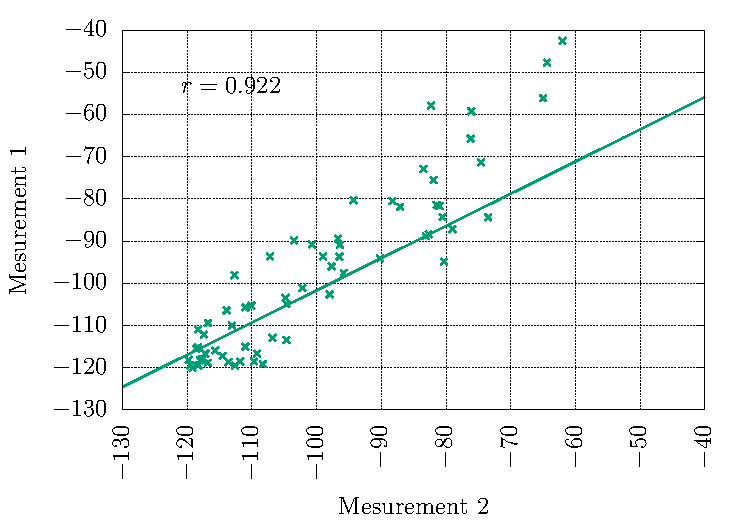
\includegraphics[width=0.8\textwidth]{./figures/Figure7/Figure7.pdf}
%   %\includegraphics[width=0.8\linewidth]{correlation2.png}
%   \caption{Comparison of RSSI values at Tomebamba river with DR$3$}
%   \label{fig:comparisonrssidr3}
% \end{figure}

The correlation value indicates that there is a strong relationship between the RSSI values. However, it does not mean that the LoRa coverage on the banks of the same river are the same, as it is shown in Section \ref{sub:compfittings}.

\begin{figure}[h!]
    \centering
      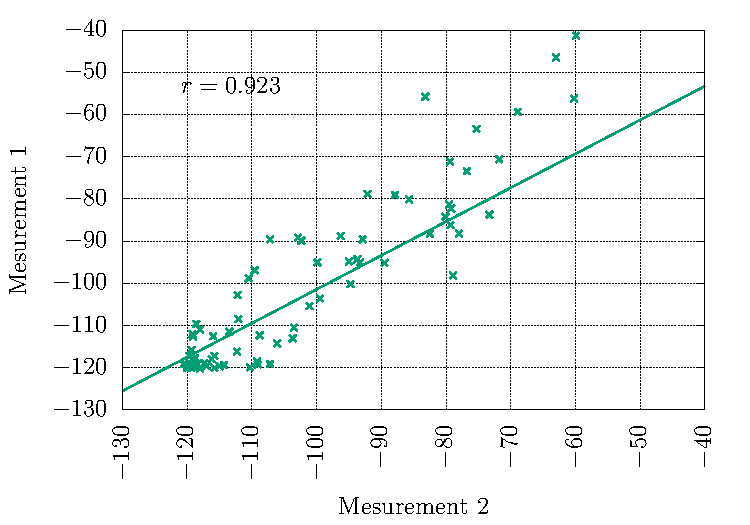
\includegraphics[width=0.9\textwidth]{./figures/Figure6/Figure6.pdf}
      \label{fig:comparisonrssidr0}
      \caption{RSSI values at Tomebamba river with DR$0$}
\end{figure}
\begin{figure}[h!]
 	\centering
      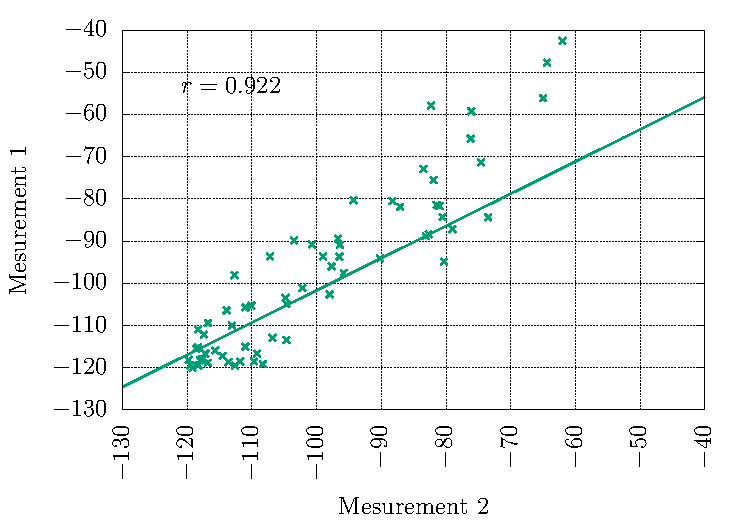
\includegraphics[width=0.9\textwidth]{./figures/Figure7/Figure7.pdf}
      \label{fig:comparisonrssidr3}
      \caption{RSSI values at Tomebamba river with DR$3$}
\end{figure}
    
\item \textbf{Distribution Comparison:} Two statistical tests were performed to determine the relationship between RSSI measurement distributions in the three selected environments. At first, the null hypothesis that the three environments had equal distributions was rejected using the Kruskal-Wallis test that resulted in a p-value of $0.01$ \cite{Mendenhall2010}.

Then, the Dunn test was performed to compare the environment combinations. These tests are focused on proving a hypothesis of equality of distributions. Table \ref{tab:testresults} presents p-values of the test. P-values shows that there is not distribution relationship between rural with semi-urban and urban with semi-urban environments.

\begin{table}[h!]
\centering
\caption{P-values of Dunn test}
\label{tab:testresults}
\begin{tabular}{@{}lrr@{}}
\toprule
\textbf{P-value}    & \textbf{Rural} & \textbf{Semi-urban}  \\ \midrule
\textbf{Semi-urban} & $0.0010$         & \multicolumn{1}{l}{} \\
\textbf{Urban}     & $0.3788$         & $0.0100$                 \\ \bottomrule
\end{tabular}
\end{table}

%However, usually the used data in these tests are not from this science area. Because there are no studies that demonstrate the applicability and validity of the results shown in this section, they must be verified in a future work.

\end{itemize}

\subsection{Path Loss Fitting}
\label{sub:fitting}

%With RSSI and SNR mean values, Equation \eqref{eq:5} was used to calculate the path loss ($P_L$). The obtained values were fitted to Equation \eqref{eq:3} using Matlab's Fit function. Finally, Equation \eqref{eq:4} was used to calculate the standard deviation.
With RSSI and SNR mean values, Equation \eqref{eq:5} was used to calculate the path loss ($P_L$). The obtained values were fitted to Eq. \eqref{eq:3}. Finally, Equation \eqref{eq:4} was used to calculate the standard deviation.

\begin{enumerate}
%[leftmargin=*,labelsep=5.8mm]

\item Propagation on Urban Environment (Measurement $1$): Figure \ref{fig:rssimeasurement} shows the RSSI measurements with DR$0$ and DR$3$. Using RSSI and SNR data, the path loss is modeled and expressed in Eq. \eqref{eq:m1dr0} and Eq. \eqref{eq:m1dr3} for DR$0$ and DR$3$ respectively. Equation \eqref{eq:m1dr3} shows less standard deviation and greater range, as shown in Tables \ref{tab:propagationcomparisondr0} and \ref{tab:propagationcomparisondr3}. The lowest standard deviation may be due to the fact that DR$3$ has fewer samples to adjust by its lower $SF$.

\begin{eqnarray} 
P_{L,DR0}(dB) = 59.53+11.26\;\log(d)+X_\theta(\theta=6.29) \label{eq:m1dr0}\\
P_{L,DR3}(dB) = 53.38+12.98\;\log(d)+X_\theta(\theta=5.12) \label{eq:m1dr3}
\end{eqnarray}

\item Propagation on Urban Environment (Measurement $2$): Compared with measurement $1$, lower standard deviations are observed in DR$0$ and DR$3$, in addition to greater coverage, this is due to the topographic characteristics of the place that are similar to those of measurement $1$ but are not the same. The logarithmic fittings are observed in Eqs. \eqref{eq:m2dr0} and \eqref{eq:m2dr3}.

\begin{eqnarray} 
P_{L,DR0}(dB) = 44.96+13.39\;\log(d)+X_\theta(\theta=5.83) \label{eq:m2dr0} \\
P_{L,DR3}(dB) = 26.24+17.49\;\log(d)+X_\theta(\theta=3.72)  \label{eq:m2dr3}
\end{eqnarray}

\item Propagation on Semi-Urban Environment (Measurement $3$): The third measurement was performed in a semi-urban environment. Standard deviations are lower compared to the urban measurements due to the lower number of obstacles in the environment. This is shown in the Eqs. \eqref{eq:m3dr0} and \eqref{eq:m3dr3}. The maximum coverage also improved to $1170$ and $1100$ meters for DR$0$ and DR$3$ respectively.

\begin{eqnarray}
P_{L,DR0}(dB) = 61.55+10.7\;\log(d)+X_\theta(\theta=2.92) \label{eq:m3dr0} \\
P_{L,DR3}(dB) = 62.74+10.67\;\log(d)+X_\theta(\theta=3.20) \label{eq:m3dr3}
\end{eqnarray}

\item Propagation on Rural Environment (Measurement $4$): The last measurement was taken in a rural setting. In this case the obstacles were mainly trees and shrubs besides the own topography of the place. The transmission range is the best since $1600$ and $1500$ meters were reached for DR$0$ and DR$3$ respectively. The logarithmic fittings are observed in Eqs. \eqref{eq:m4dr0} and \eqref{eq:m4dr3}.

\begin{eqnarray} 
P_{L,DR0}(dB) = 55.36+11.27\;\log(d)+X_\theta(\theta=3.73) \label{eq:m4dr0} \\
P_{L,DR3}(dB) = 61.13+10.55\;\log(d)+X_\theta(\theta=3.88) \label{eq:m4dr3}
\end{eqnarray}

\end{enumerate}

\subsection{Comparison of Fittings}
\label{sub:compfittings}
This section summarizes the comparison of the four measurements performed. The results show that the urban environment is the one that would need a greater number of nodes to build a network with LoRaWAN technology.

\begin{itemize}
%[leftmargin=*,labelsep=5.8mm]

\item \textbf{Measurements with the Minimum Data Rate:} Figure \ref{fig:allfitteddr0} shows a comparison of the path losses for the measured environments. It can be observed that the rural environment has the largest range. In the same way, it also can be observed that the measurement $1$, corresponding to the urban environment decays faster, as expected.

\begin{figure}[h!]
  \centering
  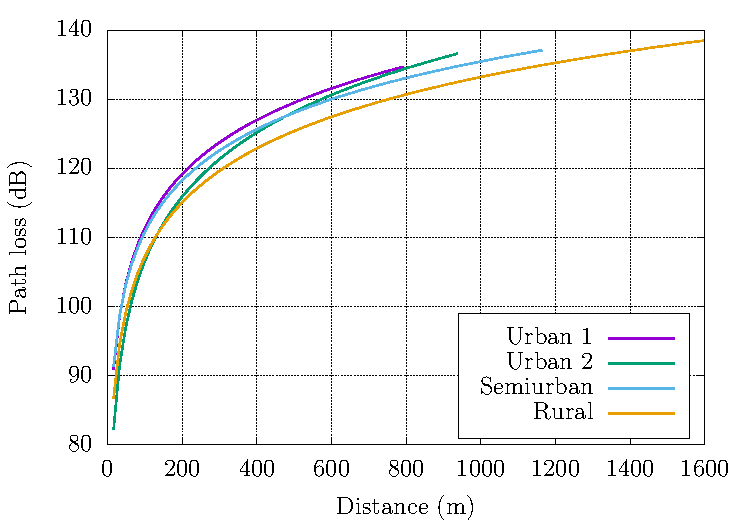
\includegraphics[width=0.9\textwidth]{./figures/Figure8/Figure8.pdf}
  %\includegraphics[width=1.1 \linewidth]{Comparacion_DR0.png}
  \caption{$P_L$ fitted models with DR$0$}
  \label{fig:allfitteddr0}
\end{figure}

The measurement $3$, corresponding to the semi-urban environment is the one with the lowest standard deviation. This indicates that it was the one that best fit the data and in which there was less shadowing as shown in the Table \ref{tab:propagationcomparisondr0}.

\begin{table}[h!]
\centering
\caption{Propagation characteristics comparison with DR$0$}
\label{tab:propagationcomparisondr0}
\begin{tabular}{@{}lrrrr@{}}
\toprule
\multicolumn{1}{c}{\textbf{Parameter}} & \multicolumn{4}{c}{\textbf{Measurement}}                                                                                          \\ \midrule
\textbf{}                              & \multicolumn{1}{c}{\textbf{Urban 1}} & \multicolumn{1}{c}{\textbf{Urban 2}} & \multicolumn{1}{c}{\textbf{Semiurban}} & \multicolumn{1}{c}{\textbf{Rural}} \\
\textbf{Max. Distance (m)}             & $800.00$                            & $950.00$                            & $1170.00$                           & $1600.00$                           \\
\textbf{Standard Deviation (dB)}       & $6.29$                           & $5.83$                           & $2.92$                           & $3.73$                           \\ \bottomrule
\end{tabular}
\end{table}


\item \textbf{Measurements with Maximum Data Rate:} The results obtained in the measurements with DR$3$ are very similar to those obtained with DR$0$ with the difference that the coverage is lower in all the measurements. The results are shown in Fig. \ref{fig:allfitteddr3} and Table \ref{tab:propagationcomparisondr3}.

\noindent
\begin{figure}[h!]
  \centering
  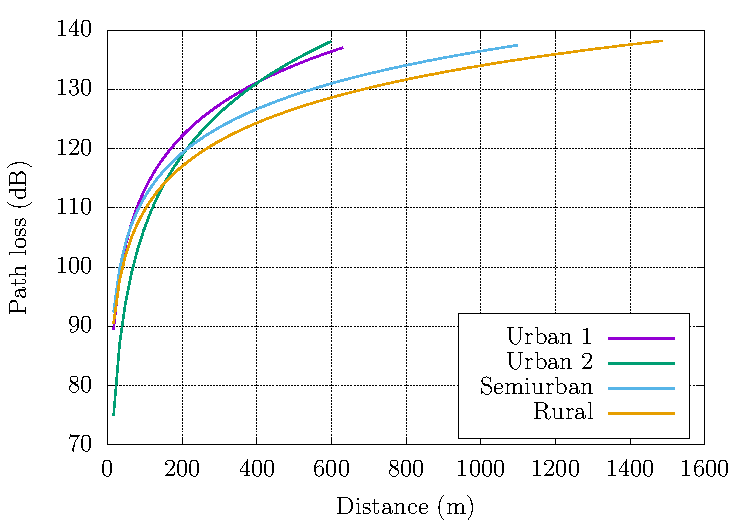
\includegraphics[width=0.9\textwidth]{./figures/Figure9/Figure9.pdf}
  %\includegraphics[width=1.1\linewidth]{Comparacion_DR3.png}
  \caption{$P_L$ fitted models with DR$3$}
  \label{fig:allfitteddr3}
\end{figure}


\begin{table}[h!]
\centering
\caption{Propagation characteristics comparison with DR$3$}
\label{tab:propagationcomparisondr3}
\begin{tabular}{@{}lrrrr@{}}
\toprule
\multicolumn{1}{c}{Parameter} & \multicolumn{4}{c}{\textbf{Measurement}}                                                                                          \\ \midrule
\textbf{}                              & \multicolumn{1}{c}{\textbf{Urban $1$}} & \multicolumn{1}{c}{\textbf{Urban $2$}} & \multicolumn{1}{c}{\textbf{Semiurban}} & \multicolumn{1}{c}{\textbf{Rural}} \\
\textbf{Max. Distance ($m$)}             & $640.00$                            & $600.00$                            & $1100.00$                           & $1500.00$                           \\
\textbf{Standard Deviation ($dB$)}       & $5.12$                           & $5.72$                           & $3.20$                           & $3.88$                           \\ \bottomrule
\end{tabular}
\end{table}

\end{itemize}


%%%%%%%%%%%%%%%%%%%%%%%%%%%%%%%%%%%%%%%%%%


\section{Conclusion and Future Work}

The transmission performance of LoRaWAN has been empirically evaluated by measuring RSSI and SNR in different riparian forested environments. The measurements found that transmission range depends strongly on the environment. The high correlation between RSSI measurements between the two banks shows a strong relationship between them. DR$0$ and DR$3$ present the same attenuation but DR$0$ presents larger range in all the measurements. Correlation Standard deviation decreases in semi-urban and rural environments due to fewer obstacles. For delivering the measurements results, the path loss characteristics have been expressed as logarithmic models.

A future work will vary transmitter and receiver antennas height to improve transmission range. Scalability in forested environments have not been proved and could present challenges to transmission with this technology. 

\small 
\section*{Abbreviations}

BW: Bandwidth; DR: Data rate; GW: Gateway; IoT: Internet of things; IP: Internet protocol; LPWAN: Low power wide area networks; LoRa: Long range; Packet error rate (PER); PROMAS (spanish abbreviation): Program for Water and Soil Management; RSSI: Received signal strength indicator; SF: Spreading factor; SNR: Signal-to-noise-ratio;  Wireless sensor network (WSN).

\section*{Funding}

This work was supported in part by the Research Department of University of Cuenca (DIUC for its acronym in spanish) under Grant 2040000-07-1278. 

\section*{Authors’ contributions}

PA designed the idea, performed the experiments, processed the data and partially written the manuscript. FA and AV verified the experiments and results, analyzed and interpreted the data and completed the writing of the manuscript. AA gave valuable suggestions on the structuring of the paper and assisted in the revising and proofreading. All authors read and agreed the manuscript. 

\section*{Competing interests}

The authors declare that they have no competing interests.

\normalsize
% use section* for acknowledgment
% \section*{Acknowledgment}
% The authors would like to thank \textit{Direcci\'on de Investigaci\'on de la Universidad de Cuenca} (DIUC) by their support.



% trigger a \newpage just before the given reference
% number - used to balance the columns on the last page
% adjust value as needed - may need to be readjusted if
% the document is modified later
%\IEEEtriggeratref{8}
% The "triggered" command can be changed if desired:
%\IEEEtriggercmd{\enlargethispage{-5in}}

% references section

% can use a bibliography generated by BibTeX as a .bbl file
% BibTeX documentation can be easily obtained at:
% http://mirror.ctan.org/biblio/bibtex/contrib/doc/
% The IEEEtran BibTeX style support page is at:
% http://www.michaelshell.org/tex/ieeetran/bibtex/
%\bibliographystyle{IEEEtran}
% argument is your BibTeX string definitions and bibliography database(s)
%\bibliography{IEEEabrv,../bib/paper}
%
% <OR> manually copy in the resultant .bbl file
% set second argument of \begin to the number of references
% (used to reserve space for the reference number labels box)
%\Urlmuskip=0mu plus 1mu\relax
\bibliographystyle{spbasic}

\bibliography{references}


% \section{Section title}
% \label{sec:1}
% Text with citations \cite{RefB} and \cite{RefJ}.
% \subsection{Subsection title}
% \label{sec:2}
% as required. Don't forget to give each section
% and subsection a unique label (see Sect.~\ref{sec:1}).
% \paragraph{Paragraph headings} Use paragraph headings as needed.
% \begin{equation}
% a^2+b^2=c^2
% \end{equation}

% % For one-column wide figures use
% \begin{figure}
% % Use the relevant command to insert your figure file.
% % For example, with the graphicx package use
%   \includegraphics{example.eps}
% % figure caption is below the figure
% \caption{Please write your figure caption here}
% \label{fig:1}       % Give a unique label
% \end{figure}
% %
% % For two-column wide figures use
% \begin{figure*}
% % Use the relevant command to insert your figure file.
% % For example, with the graphicx package use
%   \includegraphics[width=0.75\textwidth]{example.eps}
% % figure caption is below the figure
% \caption{Please write your figure caption here}
% \label{fig:2}       % Give a unique label
% \end{figure*}
% %
% % For tables use
% \begin{table}
% % table caption is above the table
% \caption{Please write your table caption here}
% \label{tab:1}       % Give a unique label
% % For LaTeX tables use
% \begin{tabular}{lll}
% \hline\noalign{\smallskip}
% first & second & third  \\
% \noalign{\smallskip}\hline\noalign{\smallskip}
% number & number & number \\
% number & number & number \\
% \noalign{\smallskip}\hline
% \end{tabular}
% \end{table}


% %\begin{acknowledgements}
% %If you'd like to thank anyone, place your comments here
% %and remove the percent signs.
% %\end{acknowledgements}

% % BibTeX users please use one of
% %\bibliographystyle{spbasic}      % basic style, author-year citations
% %\bibliographystyle{spmpsci}      % mathematics and physical sciences
% %\bibliographystyle{spphys}       % APS-like style for physics
% %\bibliography{}   % name your BibTeX data base

% Non-BibTeX users please use
% \begin{thebibliography}{}
% %
% % and use \bibitem to create references. Consult the Instructions
% % for authors for reference list style.
% %
% \bibitem{RefJ}
% % Format for Journal Reference
% Author, Article title, Journal, Volume, page numbers (year)
% % Format for books
% \bibitem{RefB}
% Author, Book title, page numbers. Publisher, place (year)
% % etc
% \end{thebibliography}

\end{document}
% end of file template.tex


%%% Local Variables:
%%% mode: latex
%%% TeX-master: t
%%% End:
